
\subsection{Science Objectives}
\label{sec:science}

\vspace{-0.05in}

\comred{5 pages for all science goals including the (temporary) two sections below.}

\subsubsection{The Inflationary Gravitational Wave Background}

\vspace{-0.05in}

% Lloyd, Sarah, Dan, Rafael
\comred{Some text recycled from placeholder/old proposal text that was here. Some text below recycled from CMB-S4 science book. Figures currently from CMB-S4.}

Inflation~\cite{guth81,linde82,albrecht82,sato81,kolb94}, a primordial era of accelerated expansion, provides a compelling dynamical origin for the observed statistical homogeneity of our universe on even the largest scales. Inflation dramatically smoothes away classical inhomogeneities, leaving the inevitable quantum fluctuations of the matter fields and the space-time metric during inflation as the source of structure today.
%Inflation is consistent with all current astrophysical measurements~\cite{spergel06,Tegmark:2006az,planck2015parameters,planck2015inflation} and is the leading paradigm for the origin of structure in the universe.  
%The statistics of the primordial curvature fluctuations depend on both the Hubble parameter during inflation and on properties of the matter that sources the fluctuations through the Einstein equation. 
The predictions of inflation are consistent with an impressive array of observations, including the cosmic microwave background temperature and E-mode polarization and many surveys of the large scale structure of the universe at later times ~\cite{spergel06,Tegmark:2006az,planck2015parameters,planck2015inflation}. But, inflation also predicts a spectrum of primordial gravitational waves sourced directly by quantum fluctuations of the tensor component of the metric. The gravitational waves in turn source B-mode polarization in the CMB fluctuations~\cite{kamionkowski97a,zaldarriaga97}. The predicted spectrum has peaks near an angular scale of $\ell=80$, and another at very low $\ell$ from the epoch of reionization. Figure \ref{fig:clall} shows the predicted spectrum, current upper limits and measured $B$-modes from lensing, as well as a range of forecasts for future satellite missions. {\bf Is this a figure we want?}

Measurements of the CMB temperature fluctuations can be used to relate the inflationary potential energy $V$ to $r$, the ratio of the temperature quadrupoles produced by gravitational waves to those from density perturbations, at the peak of the spectrum by $V^{1/4} = 3.7 \times 10^{16} \ r^{1/4}\,\, {\rm GeV}$. The observation of an all-sky, statistically homogeneous gravitational wave background would generate a revolution in our understanding the origin of our universe and the nature of particle physics, including gravity, at and above the Grand Unification scale of $10^{16}$~GeV.  In its recent report New Worlds New Horizons (NWNH), the decadal survey committee strongly endorsed sub-orbital searches for the B-mode signal from inflation saying that ``The convincing detection of B-mode polarization in the CMB produced in the epoch of reionization would represent a watershed discovery.''~\cite{blandford2010}.

\begin{figure}[h]
\begin{center}
\includegraphics[width=4in]{figs/cmb_powspec_v4.pdf}
\end{center}
\caption{Theoretical predictions for the temperature (black), 
E-mode (red), and tensor B-mode (blue) power spectra. Primordial 
B-mode spectra are shown for two representative values of the tensor-to-scalar
ratio: $r=0.001$ and $r=0.05.$ 
The contribution to tensor B modes from scattering at recombination peaks at $\ell \sim 80$
and from reionization at $\ell < 10$.
Also shown are expected values for the contribution to B modes from gravitationally lensed E modes (green).
Current measurements of the B-mode spectrum are shown for {BICEP}2/{\em Keck Array} (light orange), POLARBEAR (orange), and SPTPol (dark orange). 
The lensing contribution to the B-mode spectrum can be partially removed by measuring the 
E and exploiting the non-Gaussian statistics of the lensing.
}
\label{fig:clall}
\end{figure}

%\begin{figure}[htbp!]
%\hspace{0.in}
%\parbox{4.2in}{ \centerline {
%\includegraphics[width=2.0in] {Figures/cmb_powspec_v4.pdf}  
%\hspace{0.1in}
%\includegraphics[width=2.0in] {Figures/nsrlabeledrp01v10s}  }  }
%\hspace{0.1in}
%\parbox{2.in}{
%\caption{ \small \setlength{\baselineskip}{0.90\baselineskip}
%    Theory and observations for the spectrum; Space of predictions from important classes of inflation models.
%\label{fig:inflation} } }   
%\vspace{-0.05in}
%\end{figure}

The predicted amplitude of the $B$-mode signal depends on the nature of the scalar sector driving inflation. Although there are many proposed inflationary scenarios, when the slow-roll expansion is valid ($\epsilon\equiv-\dot{H}/H^2\ll1$) there are just two observationally viable classes of models that naturally explain the value of the spectral index $n_s$ (by requiring $n_{\rm s}(\mathcal{N})-1\propto-\frac{1}{\mathcal{N}}$, where $\mathcal{N}$ is the number of e-folds between the scale $n_s$ where is observed and end of inflation)~\cite{Mukhanov:2013tua,Roest:2013fha,Creminelli:2014nqa}. One class is the set of monomial potentials, which contains many of the canonical inflation models (eg, a quadratic potential) and is already under significant observatinoal pressure. If the error bars on the spectral index tighten by a factor of about 2, and the 95\% C.L. upper limit on $r$ is pushed down to about 0.01, all such models would be ruled out (see Figure \ref{fig:nsrp01}.). The remaining class of natural models includes Starobinsky and Higgs inflation (which have $r\sim0.003$). A future mission capable of reaching $\sigma_r\sim\mathcal{O}(10^{-4})$ would provide significant constraints on nearly every currently favored inflation model.
\begin{figure}[ht]
\begin{center}
\includegraphics[width=6in]{figs/nsrlabeledrp01v10s}
\end{center}
\caption{{\bf Perhaps a version of this figure?} Forecast of CMB-S4 constraints in the $n_{\rm s}$--$r$ plane for a fiducial model with $r=0.01$. Constraints 
on $r$ are derived from the expected CMB-S4 sensitivity to the B-mode power spectrum as described in 
Section~\ref{sec:needs}. Constraints on $n_{\rm s}$ are derived from expected CMB-S4 sensitivity to temperature and 
E-mode power spectra as described in Section~\ref{sec:ttee}. Also shown are the current best constraints from a combination of the { BICEP}2/{\em Keck Array} experiments and \planck\ \cite{Array:2015xqh}. Chaotic inflation with $V(\phi)=\mu^{4-p}\phi^p$ for \mbox{$p=2/3,1,2$} are shown as blue lines for $47<N_\star<57$ (with smaller $N_\star$ predicting lower values of $n_{\rm s}$). The Starobinsky model and Higgs inflation are shown as small and large filled orange circles, respectively. The lines show the classes of models discussed in Section~\ref{sec:upperLimits}. The green band shows the predictions for quartic hilltop models, and the gray band shows the prediction of a sub-class of $\alpha$-attractor models~\cite{Kallosh:2013hoa}.
}
\label{fig:nsrp01}
\end{figure}

Forecasts for the capability of a variety of configurations for a future satellite mission (including PIXIE, LiteBird, CORE+, EPIC-2m) are reported to find $\sigma(r)\sim4 \times 10^{-4}$ assuming $r=0.01$, and $\sigma(r)\sim2\times 10^{-4}$ for $r=0$. {\bf Do we want a figure of $\sigma(r)$ versus something? A figure/table with some example specs and $\sigma(r)$?}

Inflation generically predicts primordial gravitational waves just from the vacuum fluctuations of the metric during inflation, but of course does not preclude additional sources of $B$-mode polarization either during or after inflation. If $B$-modes are detected, it would be important to characterize the signal to rule out the possibility of a non-inflationary source. 
%The standard inflationary prediction is distinguished in these cases by several things: an extremely Gaussian, nearly scale-invariant spectrum with a slight red tilt, the presence of correlations on scales that were not in causal contact at the time of recombination. 
The vast majority of inflation scenarios predict a red spectrum for gravitational waves, and in the simplest cases the canonical single-field consistency relation fixes $n_{\rm t}=-r/8$. While confirming this relation is out of reach, a future mission could perhaps aim for $\sigma(n_{\rm t})\sim1${\bf ??} to at least rule out non-vacuum inflationary sources  \cite{Namba:2015gja,Peloso:2016gqs}. Post-inflationary phase transitions have been proposed as a non-inflationary source of nearly scale-invariant gravitational waves \cite{Krauss:1991qu,JonesSmith:2007ne,Giblin:2011yh,Figueroa:2012kw,Fenu:2013tea}, but can be distinguished by the absence of super-horizon correlations at the time of recombination. A framework to extract specifically this part of the signal was proposed in Ref.~\cite{Baumann:2009mq} and could be applied to robustly extract the component of any signal that must come from physics outside of the hot big bang paradigm. Existing forecasts in the literature \cite{Lee:2014cya} indicate that a ground-based survey alone will not be able to detect super-horizon correlations at high significance if $r$ is much below $0.1$; a satellite will be required.

A detection of $B$-modes consistent with a primordial spectrum of vacuum fluctuations would be the first observation of a phenomena directly related to quantum gravity. In addition, evidence for ``large field" inflation would provide strong evidence that the complete theory of quantum gravity must accommodate a Planckian field range for the inflaton. The spectrum of tensor fluctuations depends only on the Hubble parameter $H$ during inflation, while the scalar power depends on both $H$ and the evolution of the homogeneous field sourcing inflation. As a consequence, the tensor-to-scalar ratio $r$ determines the inflaton field range in Planck units (called the ``Lyth bound'' \cite{Lyth:1996im})
%\begin{equation}
%\label{eq:Lyth}
%\frac{\Delta\phi}{M_{\rm P}}=\int_0^{\mathcal{N}_\ast}d\mathcal{N}\,\left(\frac{r}{8}\right)^{1/2}\,,
%\end{equation}
%where (applying the general equation to the observationally accessible regime) $\mathcal{N}_\ast$ is the number of e-folds between the end of inflation and the moment when the mode with $k_\ast=0.05\,{\rm Mpc^{-1}}$ (corresponding to the CMB pivot scale) exits the horizon. 
In many common inflationary models $r$ is a monotonic function of $\mathcal{N}$ so that the tensor-to-scalar ratio at the CMB pivot point $k_*$ is related to the distance the inflaton moves ($\delta\phi$) in Planck units by
\begin{equation}
\label{eq:lbound}
\frac{\Delta\phi}{M_{\rm P}}\gtrsim \left(\frac{r_\ast}{8}\right)^{1/2}\mathcal{N}_\ast\gtrsim \left(\frac{r}{0.01}\right)^{1/2}\,.
\end{equation}  
The value of $\mathcal{N}_\ast$ is not well constrained and depends on unknown details of reheating, but $\mathcal{N}_\ast\gtrsim 30$ provides a conservative lower limit, justifying the second inequality in Eq.~(\ref{eq:lbound}). Thus, a tensor-to-scalar ratio $r>10^{-2}$ typically corresponds to a trans-Planckian excursion in field space between the end of inflation and the epoch when the modes we observe in the CMB exit the horizon. The relationship in Eq.~(\ref{eq:lbound}) is significant because it relates the observed amplitude of linearized metric fluctuations to a property of the full quantum field theory for gravity coupled to the inflaton. The action describing inflation, like the action for any other particle physics phenomena, in general will include terms that encode the effects from degrees of freedom that couple to the inflaton, but are too energetic to be probed directly by physics near the inflationary scale. The field range is a measure of the distance in field space over which the corrections from the unknown physics do not significantly affect the low energy dynamics, since otherwise slow-roll inflation would not persist. In theories of quantum gravity we expect degrees of freedom to enter at the Planck scale or below. A field range exceeding the Planck scale would imply that quantum gravity contributions do not have a significant effect over the naively expected scale. A detection of $r$ would therefore provide very strong motivation to better understand how ``large-field inflation" can be naturally incorporated in quantum gravity.

Although the $B$-mode polarization is the richest source of new information, deeper mapping of $E$-mode polarization will also contribute to testing inflationary models. On the largest scales (accessible only from space), $E$-modes will provide new tests of isotropy, while on sufficiently small scales they will allow tighter constraints on the shape of the scalar power spectrum, the amplitude of scalar non-Gaussianities, and isocurvature modes.  

In summary, a detection of primordial gravitational waves consistent with the standard inflationary prediction would reveal the presence of a new fundamental energy scale for particle physics and would have far reaching implications for quantum gravity. Detecting correlations on the largest scales would confirm a primordial origin. Any departure from a nearly scale-invariant, nearly Gaussian spectrum would reveal new physics beyond the simplest inflationary model. In the absence of a detection, an improvement by a factor of xxx in the upper limit would qualitatively change how we think about the inflationary paradigm.

\vspace{-0.15in}

\subsubsection{Neutrinos and Light Relics}

\vspace{-0.05in}

Much of the information about our thermal history and the particle content of the universe is encoded in the $T$ and $E$ power spectra.  
A high-precision measurement of these spectra over the full sky is expected to significantly improve our understanding of the post-inflationary 
universe.  This is particularly true in $E$-mode polarization where, to date, far fewer modes have be measured at the level of cosmic variance than in temperature.

The spectra at high-$\ell$ contain important information about the components of the thermal plasma and their interactions around the time of recombination.  One particular compelling target is the effective number of neutrino species, $\Neff$, which parameterizes the total amount of energy density in radiation at the time of recombination.  It is defined such that in the Standard model of particle physics with normal thermal evolution, $\Neff = 3.046$ due to the energy density in the three species of neutrinos.  $\Neff$ is also sensitive to any additional light relic particles as their gravitational influence is identical to the neutrinos.  In fact, if there was an additional light particle in thermal equilibrium with the Standard model particles at any point in our history, it will contribute a change to $\Neff$ of at least $\Delta \Neff \geq g \, 0.027$ where $g \geq 1$ is the number of degrees of freedom of the new particle.  This defines a compelling target of $\sigma(\Neff) < 0.027$ for future CMB observations.  New light particles are a common feature of many approaches to beyond the Standard model physics and can be directly tied to some of the most significant problems in the Standard model.  Either a limit or detection of $\Delta \Neff$ at this level would provide a powerful insight into the laws of nature and our thermal history. 

The presence of free-streaming radiation changes the detailed features of the $TT$, $TE$ and $EE$ spectra at all $\ell$.  In particular, it changes the locations of the acoustic peaks and alters the damping tail at high-$\ell$.  Similar changes to the spectra arise from many other compelling targets including the helium fraction $Y_p$ and more general dark sector physics.  For this reason, constraints on $\Neff$ a useful proxy for the information available in the high-$\ell$ power spectra.  

Preliminary forecasts for $\Neff$ are shown in the right hand panel of Figure~\ref{fig:Neff_future}.  A space-based mission reaching an effective temperature noise of 1-2 $\mu$K-arcmin over the full sky gives competitive constraining power when compared other proposals.  The two most important quantities for improving constraints on $\Neff$ and other high-$\ell$ targets are $f_{\rm sky}$ and the temperature noise.  The full-sky nature of the proposed mission would allow for cosmic variance limited $E$-modes over most of the sky and a large range of $\ell$.

The main downside of a space-based mission is that we cannot reach the resolutions available from the ground.  However, we see that at 5' resolution and 1 $\mu$K-arcminute noise the forecasts are less sensitive to the resolution then one might naively expected.  In particular we can reach $\sigma(\Neff) < 0.035$ for temperature noise from 1-2 $\mu$K-arcmin and $f_{\rm sky} =0.6-0.8$.  These forecasts are competitive with CMB Stage IV.  Specifically, the larger sky fraction and sensitivity available from space appears to compensate for the reduced resolution.  In fact, the full sky measurement would provide complimentary information that could be combined with ground based surveys to further improve over the limits available from either experiment.  This is particularly important for $\Neff$ which is tantalizingly close to the target of $\sigma(\Neff) =0.027$ and therefore even an apparently modest improvement could have a major scientific impact.  

The sum of neutrino masses, $\sum m_\nu$, is another theoretically compelling target that is accessible from Cosmology.  The most distinctive feature of $\sum m_\nu$ is that it suppresses the growth of structure on small scales.  This suppressed can be measure in the CMB through amplitude of the lensing power spectra compared to the primary CMB.  In principle, this relative difference can yield a measurement  of the minimum value of $\sum m_\nu =58$ meV at 4-5 $\sigma$ for a number of future cosmological surveys.  However, sensitivity to $\sum m_\nu$ is ultimately limited by our knowledge of the primordial amplitude of fluctuations $A_s$ which is strongly degenerate with the optical depth $\tau$. 

The current limit on $\tau$ from the Planck satellite of $\tau = 0.055 \pm 0.009$ ultimately limits $\sigma(\sum m_\nu) \gtrsim 25$ meV, as shown in the panel of Figure~\ref{fig:Neff_future}.  While the figure shows the sensitivity of a space-based CMB mission to $\sum m_\nu$, this lower limit is common to any measurement that depends on the relative suppression.  Therefore, a cosmological detection of $\sum m_\nu = 58$ meV at 3-5 $\sigma$ depends crucially on an improvement measurement of $\tau$.  To date, the only proven method for such a measurement is from a space-based CMB observations.  The best constraints on $\tau$ come from $E$-modes with $\ell < 20$ which requires control over the largest angular scales.  


\begin{figure}[t!]
\begin{center}
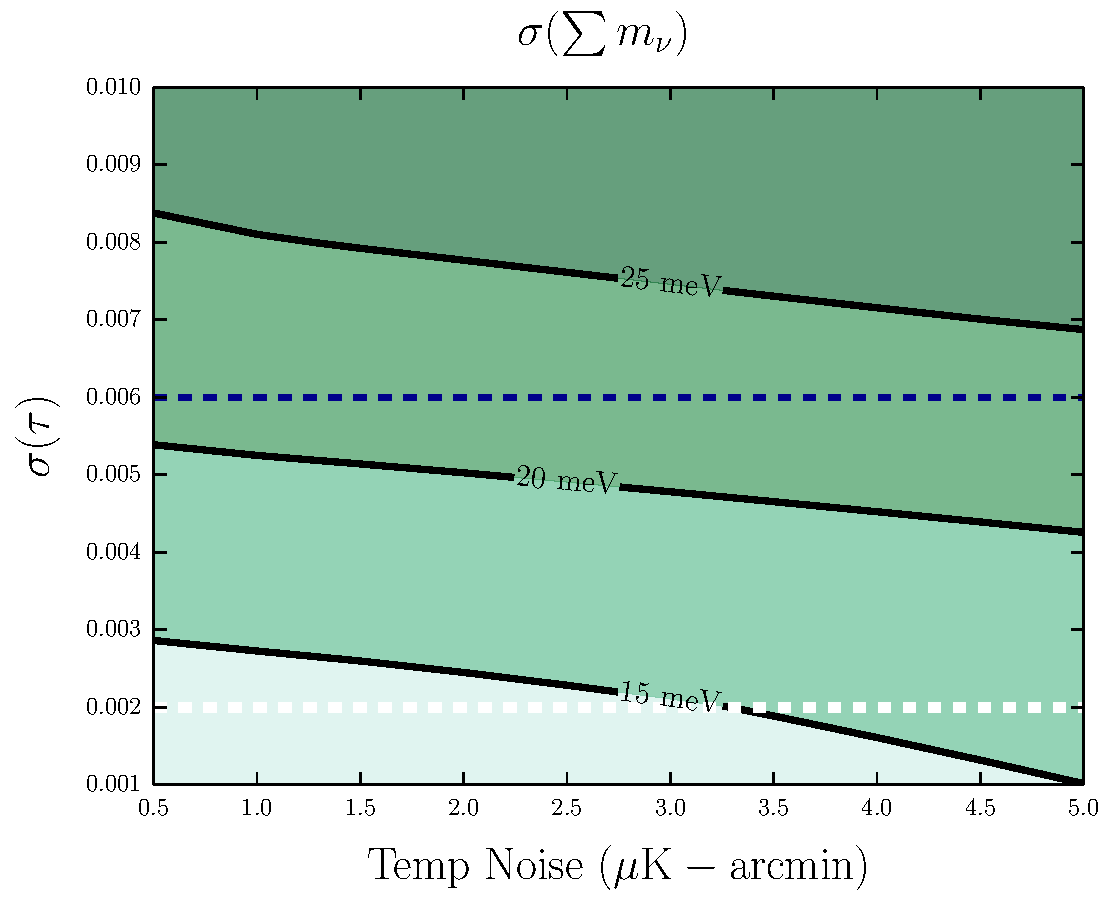
\includegraphics[width=0.45\textwidth]{figs/Mnu_tauprior.pdf}
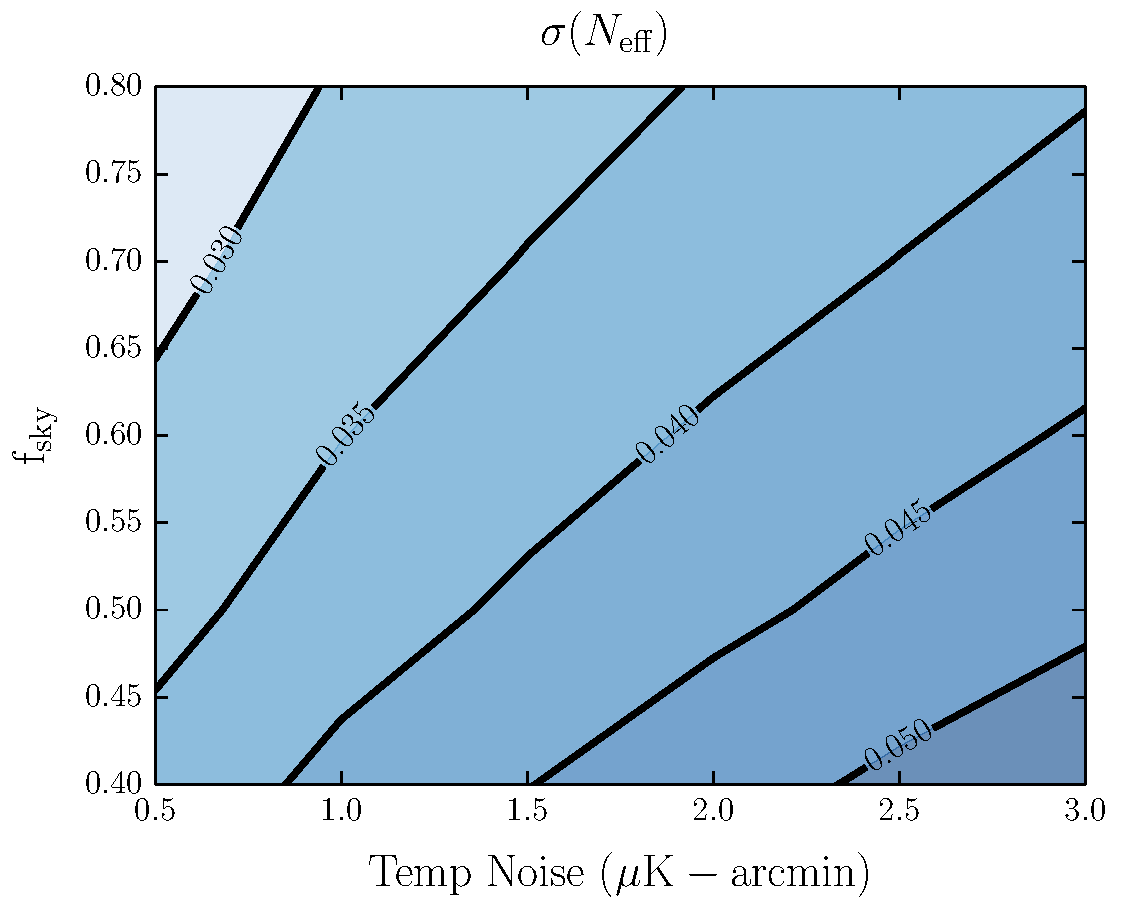
\includegraphics[width=0.45\textwidth]{figs/Neff.pdf}
\caption{ {\it Left:} Neutrino mass constraints as a function of the prior on $\tau$ for a 5' beam and sky fraction of $f_{\rm sky} = 0.7$.  The blue dashed line is the Planck blue book expectation and the white dashed line a cosmic variance limit measurement of $\tau$ form the CMB. {\it Right:} $\Neff$ Forecasts as a function temperature noise and sky fraction assuming 5' resolution.}
\label{fig:Neff_future}
\end{center}
\end{figure}


\vspace{-0.15in}
\subsubsection{CMB spectral distortion science}
\vspace{-0.05in}

In addition to the CMB temperature and polarization anisotropy targeted by CMB imagers, {\it unique} new information about 
early-universe physics can be gained by studying the energy spectrum of the 
CMB~\citep{Sunyaev1970SPEC, Burigana1993, Hu1993, Chluba2011therm}. The measurements of COBE/FIRAS have shown that 
the average CMB spectrum is consistent with that of a blackbody to an accuracy of 4 parts in $10^{4}$: 
$T_0=(2.726\pm 0.001)\,{\rm K}$~\citep{Mather1994, Fixsen1996}. These are the best measurements
of the average spectrum to date. However, several standard processes that encode 
unique information about the Universe are expected to {\it distort} 
the CMB spectrum \citep[e.g.,][]{Chluba2016LCDM} at a level that is within reach of present-day technology \citep{Kogut2011PIXIE, PRISM2013WPII}. 
%
The classical distortion shapes arise from inverse Compton scattering and chemical potential changes~\citep{Zeldovich1969, Sunyaev1970mu}, 
commonly denoted as $y$- and $\mu$-type distortions, respectively, and are caused by energy exchange of CMB photons with free electrons. 
A $\mu$-distortion can only be produced in the hot and dense environment present at redshifts $z\gtrsim 5\times10^4$, while $y$-type 
distortions are caused at lower redshifts. This makes $\mu$-distortions a unique messenger from the early Universe. 

{\bf $y$ Distortion:} The largest guaranteed distortion is caused by the late-time energy release of forming structures and 
from reionization \citep{Sunyaev1972b, Hu1994pert, Oh2003, Cen1999, Refregier2000}, imprinting a $y$-type distortion 
with $y \simeq 2\times 10^{-6}$ \citep[e.g.,][]{Refregier2000, Hill2015}. This distortion is only one order of magnitude below the current limit 
from COBE/FIRAS and, even with most pessimistic assumptions about foregrounds, should be clearly detected with the next-generation 
spectrometers we propose to study. A detection will give information about the total energy output of first stars, AGN and galaxy clusters. 
In particular, group-size clusters that have masses $M\simeq 10^{13}\,M_{\odot}$ contribute significantly to the signal. 
With temperature $k T_{\rm e}\simeq 1\,{\rm keV}$ these are still sufficiently 
hot to create a detectable relativistic temperature correction to the large $y$-distortion, 
which will be used to constrain the currently uncertain feedback mechanisms used in hydrodynamical simulations
of cosmic structure formation~\citep{Hill2015}. These two inevitable signals probe the low-redshift 
Universe and provide clear targets for future spectral distortions measurements and their requirements in the presence of foregrounds.

{\bf $\mu$ Distortion:} Next generation CMB spectrometers are also expected to greatly improve the $\mu$-distortion 
limits of COBE/FIRAS \citep{Kogut2011PIXIE}. This will allow us to place stringent bounds on the presence of long-lived decaying 
particles \citep{Hu1993b, Chluba2013fore, Chluba2013PCA, Dimastrogiovanni2015} and other new 
physics \citep[e.g.,][]{Jedamzik2000, Tashiro2012, Dolgov2013, Tashiro2013, Caldwell2013, Yacine2015DM}, but a clear target is 
predicted by the dissipation of small-scale perturbation through Silk-damping \citep{Sunyaev1970diss, Daly1991, Hu1994, Chluba2012}. 
This process allows us to place stringent constraints on the amplitude of the small-scale curvature power spectrum, present at 
scales (wavelength $0.1 \,{\rm kpc} \lesssim \lambda \lesssim 1\, {\rm Mpc}$) and epochs ($10^4 \lesssim z\lesssim 10^6$) 
inaccessible through any other observation. This delivers a complementary test for the inflation 
paradigm~\citep{Chluba2012inflaton, Dent2012, Chluba2013PCA, Clesse2014, Cabass2016}, with $\mu=(2.0\pm0.14)\times 10^{-8}$ 
expected in $\Lambda$CDM \citep{Chluba2016LCDM}. Precise measurements of signals at this level will be extremely challenging 
and requires unprecedented control of systematics and modeling of foregrounds. It would also bring us to the sensitivity level required 
to detect the cosmological recombination radiation \citep{Sunyaev2009, Chluba2016} imprinted by the recombination of hydrogen 
and helium at redshift $z\simeq 10^3-10^4$. Optimizing next-generation CMB spectrometers for these purposes requires extensive studies.
\comred{how about a plot showing required sensitivity and lines showing the reach of a \$250M and \$700M missions?}

The CMB spectrum also varies spatially across the sky. One source of such anisotropic distortion is related to clusters of galaxies 
and has already been measured by Planck~\citep{Planck2013SZ}. A combination of precise CMB imaging and spectroscopic measurements 
will allow observing the relativistic temperature correction of individual SZ clusters~\citep{Sazonov1998, Itoh98, Challinor98}, which 
will calibrate cluster scaling relations and inform our knowledge of the dynamical state of the cluster atmosphere. 
Anisotropy in the $\mu$-distortion can 
be created through `ultra-squeezed limit' non-Gaussianity~\citep{Pajer2012, Ganc2012} and will be used to probe 
scale-dependent non-Gaussianity~\citep{Biagetti2013, Razi2015}. Finally, resonant scattering signals in the 
recombination~\citep{Jose2005, Carlos2007Pol, Lewis2013} and post-recombination 
eras~\citep{Kaustuv2004, Schleicher2008} can lead to spectral-spatial CMB signals that can be used to constrain the 
presence of metals in the dark ages and the physics of recombination. For all these applications, instrumental synergies between 
CMB imaging and spectroscopy need to be studied in detail. 

Future space-borne studies of the CMB spectrum open a new window to early phases of the Universe ($z > 10^3$), 
which cannot be probed in any other way. This yet unexplored tool for testing the standard cosmological paradigm 
including inflation and reionization, 
as well as a host of non-standard physical mechanisms, such as decaying an annihilating particles, 
can {\it only} be exploited with a satellite mission. 

%This will not only allow us to test  (e.g., inflation and reionization) 
%but also opens up a huge discovery space to non-standard physics (e.g., decaying/annihilating particles). This immense potential and 
%complementarity with CMB anisotropy studies makes CMB spectral distortions an important future target and identifying experimental 
%routes towards extracting these tiny signals from the early Universe will be one main objective of the proposed mission study.

\vspace{-0.15in}
\subsubsection{The Cosmic Infrared Background}
\vspace{-0.05in}
A significant contamination of CMB anisotropy maps is due to
the foreground emission from infrared (IR)
galaxies, responsible for the cosmic infrared background (CIB).
The CIB is the second largest
extragalactic background after the CMB, with an approximate
brightness of 24 nW m$\mathrm{^{-2} sr^{-1}}$ \citep{dole2006}.
Dust enshrouding star-forming galaxies at high redshift
is heated by starlight at ultraviolet (UV) and optical wavelengths,
and re-radiates at mid-IR to sub-millimetre wavelengths.
Thus, the integrated emission from galaxies actively
producing stars at the peak of star formation
($\mathrm{z\sim 1-3}$) reaches us in the far-infrared (FIR) regime,
carrying a wealth of information about the the evolution of
large-scale structures and the history of star formation.
While the CIB is not our only handle on the evolution of the
cosmic star formation rate (SFR), it is particularly important
because FIR/sub-millimetre surveys are not subjected to some
uncertain steps in the conversion from galaxy counts and luminosities to SFRs,
affecting, e.g., optical surveys.

The drawback of working with a
high density of faint, distant sources in the FIR regime is that
individual objects are blended. While both the {\it Herschel} and {\it Planck} satellites
recently performed ground-breaking measurements of the CIB
\citep{amblard2011,viero2013a,planck2014-XXX,mak2016}, only a
negligible fraction of {\it Planck} sources have been individually
identified, due to its poor angular resolution, while for
{\it Herschel} maps, only 10$\%$ of the objects
has been resolved into individual galaxies at 857 GHz \cite{bethermin2010}.
However, the anisotropies detected in the
unresolved background can be analyzed through statistical tools
such as the angular power spectrum \citep{knox2001} and, since they trace the
underlying dark matter field, they can be interpreted with
phenomenological models linking dark matter halos to IR galaxies,
such as the Halo Model \cite{cooray2002,shang2012}.

The Planck Collaboration, analyzing CIB anisotropies and their
correlation with CMB lensing \citep{planck2014-XXX,planckXVIII},
derived limits on the star formation rate density that,
at redshift $\mathrm{z>2}$, are higher than what found from the analysis of
different datasets (see for example \cite{madau2014}).
Clearly, more accurate measurements of the CIB clustering at the
angular scales probed by {\it Planck} will be extremely useful to
gain more insight on the evolution of the star formation rate at
high redshift. The new mission probe will measure CIB anisotropies
with only one tenth of {\it Planck}'s instrumental noise at the critical
scales where the clustering of galaxies in the same dark matter
halo (the 1-halo term) has the same amplitude as the
clustering due to galaxies in separated halos
(the 2-halo term). Assuming a precise knowledge of the
Poisson level of CIB
galaxies, we will be able to firmly
constrain our models of CIB clustering,
and thus address three of the seven key questions
identified in the Astro2010 report
``New Worlds, New Horizons in Astronomy and Astrophysics''
(NAS Decadal Survey, p. 47):
{\it What is the fossil record of galaxy assembly                                                   
from the first stars to present? What are the connections                                           
between dark and luminous matter?
How do cosmic structures form and evolve?}

However, constraining the history of star formation is not the only reason for
measuring CIB anisotropies with increased sensitivity
from very large to very small scales. Below, we briefly discuss some others.
\begin{itemize}
\item The CIB is an important foreground for CMB studies. As shown in
\cite{planck2016like}, a significant contribution to the
astrophysical foreground in the 143x217 and 217x217 GHz channels is
due to both the clustering and Poisson components of the CIB.
The cross-correlation between IR galaxies and the thermal
Sunyaev-Zeldovich (tSZ) effect provides an additional contamination.
Thus, an accurate determination of both CIB and CIB-tSZ power
spectra will be extremely useful when accounting for these foregrounds
in the CMB parameter estimation.
\item The CIB, being a tracer of the dark matter field over a broad redshift range,
can be cross-correlatated with many other datasets to explore
the interplay between CIB galaxies and dark matter. Beyond the
cross-correlation with the lensing of the CMB
\citep{planckXVIII,holder2013}, some other examples include the cross-correlations
with catalogs of quasars \citep{wang2015} and
galaxies \citep{serra2014} to constrain the interplay between
SFR and halo mass, and the cross-correlation with the Cosmic
$\mathrm{\gamma}$-ray background from {\it Fermi}-LAT
\citep{fermi2016} to constrain the dark matter annihilation
cross-section \citep{cooray2016}.
\item Since they are both tracers of the underlying mass distribution over
a broad range of redshifts, the CIB and CMB lensing are highly correlated
\citep{planckXVIII}. In particular, the CIB can be used as
an ideal proxy for the CMB lensing field in delensing studies, aiming at
reducing the confusion due to B-modes from lensing in the search of the
signal from primordial gravitational waves.
Recently \cite{sherwin2015,larsen2016} showed that co-adding {\it Planck} CIB maps
greatly improves the delensing performance. Upcoming CMB surveys
will heavily rely on delensing methods for constraining the
inflationary B-mode polarization signal, and CIB delensing of temperature and E-mode
polarization might also help improving constraints on other parameters such as the effective
number of neutrino species $\mathrm{N_{eff}}$ \citep{larsen2016}.
\end{itemize}
To summarize, the CIB is a full sky, bright, high redshift extragalactic
background that maps star formation at its peak, and carries
a tremendous amount of information about the birth and
evolution large scale structures in the Universe, and the interplay
between light and matter.


% 
%
% Some of the most important information is on the largest scales: super-horizon correlations
% What do we learn: new energy scale for fundamental phenomena in particle physics; energy scale of inflation/Hubble parameter during inflation; field range and q. grav; classes of inflationary potentials; with a detection, can go after shape of the spectrum, NG. These constrain non-minimal inflation models (secondary sources), spectrum of physics BSM through cosmic strings; Any alternatives to inflation or to Einstein gravity (massive gravity, etc) must be consistent with the measured spectrum.  
% any additional power for scalar sector?
 
 %***********************  The placeholder text is below ***************************%
%\comred{The verbiage below is taken from another proposal. Here we need to explain what are the science objectives 
%of the CMBProbe, how the science objectives relate to the current state of knowledge, and to NASA's goals}
%
%
%The paradigm of inflation~\cite{guth81,linde82,albrecht82,sato81,kolb94}
%%, in which the Universe underwent exponential expansion within the first $\sim$$10^{-35}$~sec, 
%makes several predictions that are consistent with all current astrophysical 
%measurements~\cite{spergel06,Tegmark:2006az,planck2015parameters,planck2015inflation}. 
%A robust prediction of inflation is the existence of a stochastic background of gravitational radiation 
%with an amplitude depending on the mechanism driving the accelerated 
%expansion~\cite{starobinsky82,starobinsky83a,rubakov82,grishchuk75,abbott84a}.
%In most scenarios, this `inflationary gravitional wave background' (\igb) is predicted
%to have a spatial power spectrum whose amplitude is proportional to the energy
%scale of inflation $V^{1/4}$ via
%$V^{1/4} = 3.7 \times 10^{16} \ r^{1/4}\,\, {\rm GeV},$
%where $V$ is the inflaton potential and $r$ is the ratio of the temperature
%quadrupoles produced by gravitional waves and by density perturbations.  
%There are theoretical reasons $V^{1/4}$ may be close to the Grand
%Unification scale of $10^{16}$~GeV, suggesting detectable $r$ values between 
%$\sim$0.001 and $\sim$0.1. In addition to determining the energy scale of inflation, measurements 
%of the \igb\ probe the scalar field potential at or above the Planck scale, which is particularly relevant for inflation models motivated 
%by string theory~\cite{SnowmassInflationTheory}. Measurements of the \igb\ thus probe fundamental physics at the 
%highest possible energy scales. 
%\begin{figure}[htbp!]
%\hspace{0.in}
%\parbox{4.2in}{ \centerline {
%
\includegraphics[width=2.0in] {Figures/sunny_skies.jpg}  
%\hspace{0.1in}
%
\includegraphics[width=2.0in] {Figures/sunny_skies2.jpg}  }  }
%\hspace{0.1in}
%\parbox{2.in}{
%\caption{ \small \setlength{\baselineskip}{0.90\baselineskip}
%       Sample Figure of Sunny Skies
%\label{fig:sunny_skies} } }   
%\vspace{-0.05in}
%\end{figure}
%
%The most promising way to search for the \igb\ is through its signature on the CMB polarization~\cite{kamionkowski97b,seljak97}.  
%Primordial energy density perturbations produce only a curl-free, or `E-mode', pattern of polarization.
%Gravitional waves also produce a curl, or `B-mode', pattern of polarization that density perturbations cannot
%produce~\cite{kamionkowski97a,zaldarriaga97}.  The amplitude of the B mode is related to the energy scale
%of inflation by $V^{1/4}=2\times10^{16} \ ( B_{peak} / 0.1\,\mu{\rm
%K})^{1/2} \,{\rm GeV},$ where $B_{peak}$ is the amplitude of the power spectrum of the B mode in \microk\ at $\ell=80$;
%see Fig.~\ref{fig:sunny_skies}. In its recent report New Worlds New Horizons (NWNH), the decadal survey 
%committee strongly endorsed sub-orbital searches for the B-mode signal from 
%inflation saying that ``The convincing detection of B-mode polarization in the CMB produced in the 
%epoch of reionization would represent a watershed discovery.''~\cite{blandford2010}
%
%B-mode signatures near the expected \igb\ peak at $\ell=80$ have recently been detected by BICEP2~\cite{bicep2Bmode}. 
%However, the combination of Planck data with those from the BICEP2 and Keck Array collaborations have demonstrated 
%that the B-mode signal measured is entirely consistent with contributions from polarized emission of Galactic dust and the 
%signal from the gravitational lensing of CMB photons by the large scale structure of the Universe (see 
%Section~\ref{sec:lensing})~\cite{bkp2015,planck2014-XXX,2016PhRvL.116c1302B}. 
%These data give an upper limit of $r<0.09$ at 95\% confidence level.
%Most importantly, the constraint is largely limited by Planck's noisy measurement of the dust properties in the 353~GHz band; 
%a noiseless dust map could shrink the constraint by a factor of two~\cite{bkp2015}. 
%Further progress --- detections or improved limits --- requires instruments 
%with higher sensitivity at {\it both} the dust and CMB frequency bands so that this Galactic foreground can be properly identified 
%and removed. 
%
%

